\setlength{\parindent}{0pt}
\chapter{\bf INTRODUCTION}

\section{UV-induced damages in humans}

Ultraviolet (\gls{uv}) light is the major cause of skin cancers in humans \citep{kiefer2007effects}. It is a portion of the electromagnetic spectrum which is emitted from the sun together with visible light and heat. Based on its wavelength, \gls{uv} light divides into three subgroups: \gls{uv}A (wavelength of 315-400 nm), \gls{uv}B (wavelength of 280-315 nm), and \gls{uv}C (wavelength of 100-280 nm). While the less energetic \gls{uv}A makes up the majority of \gls{uv} light passing the atmosphere, all \gls{uv}C and approximately 90\% of \gls{uv}B is either blocked or absorbed by the ozone layer. Even in these conditions, humans are not fully protected from the damaging effects of \gls{uv} light. So that, \gls{uv}-irradiation accounts for approximately 30.000 \gls{dna} lesions’ formation per cell per hour.

The most abundant \gls{uv} lesions in cellular \gls{dna} are pyrimidine dimers \citep{kielbassa1997wavelength}, which are formed by the covalent bonds between the adjacent pyrimidines \citep{whitmore2001effect}. Different in their chemical structure, two types of pyrimidine dimers are exist; one is called cyclobutene pyrimidine dimers (\gls{CPD}s), and the other is called pyrimidine (6-4) pyrimidone photoproducts [\gls{64}s]. While both \gls{uv}C and \gls{uv}B can induce these dimer formations, \gls{uv}A is only capable of inducing \gls{CPD}s. Nonetheless, \gls{uv}A induction can convert already formed \gls{64}s into their Dewar valence isomers. Moreover, \gls{uv}A can induce oxidative \gls{dna} damages through photosensitized reactions \citep{hu2017cartography}. Thanks to the development of time resolved spectroscopy techniques in recent years, dynamics of pyrimidine dimer formation is well known. The formation and biological properties of \gls{uv} lesions will be briefly discussed in the subsections below.   

\subsection{Cyclobutene pyrimidine dimers (CPDs)} 

\gls{CPD}s are the most frequent pyrimidine dimers that are arising from the covalent linkages between the consecutive pyrimidines, and it is characterized by the four-member ring structure that are double bonded from the pyrimidine 5 and 6 \citep{whitmore2001effect}. In vivo, \gls{CPD}s can be observed in four different configurations: cis-syn, cis-anti, trans-syn, or trans-anti. \citep{khattak1972photochemical} While it is generally observed in cis-syn form when the \gls{dna} is double-stranded \citep{wacker1964organic}, in denatured \gls{dna} and single-stranded regions, trans-syn configuration exists \citep{taylor1988synthesis}. Although it is rare, nonadjacent pyrimidines can also form \gls{CPD}s in single-stranded regions \citep{nguyen1988ultraviolet}. Moreover, different configurations can affect the ability of repair enzymes to recognize these lesions and correct them, which cause mutability differences between the configurations \citep{friedberg2005dna}. 

Apart from the configuration of the lesions, their dipyrimidine doublets (\gls{T}\gls{T}, \gls{T}\gls{C}, \gls{C}\gls{T}, and \gls{C}\gls{C}) can contribute to \gls{CPD} formation at different rates depending on the type of \gls{uv} exposure or the nucleotide content of the \gls{dna}. According to the study of Douki and Cadet, under \gls{uv}C and \gls{uv}B exposure, double-stranded mammalian \gls{dna} produces \gls{T}\gls{T}, \gls{T}\gls{C}, \gls{C}\gls{T}, and \gls{C}\gls{C} \gls{CPD}s in 100:50:25:10 ratios, respectively \citep{douki2001individual}. While \gls{T}\gls{T} \gls{CPD}s accounts for more than half of the total \gls{CPD}s after the exposure of \gls{uv}C and \gls{uv}B, for \gls{uv}A exposure, this ratio rises to 90\% \citep{mouret2010uva}. On the other hand, \gls{T}\gls{T} \gls{CPD}s are the abundant products of \gls{uv} exposure for mammalian \gls{dna}, but the abundance might be greatly influenced by the \gls{G}\gls{C} percentage of the \gls{dna}. For example, in the bacterial \gls{dna} that possess a rich \gls{G}\gls{C} percentage, \gls{T}\gls{T} \gls{CPD}s are the minor products of \gls{uv} exposure \citep{patrick1977studies}.

\subsection{Pyrimidine (6-4) pyrimidone photoproducts [(6-4)PPs] and their Dewar valence isomers}

\gls{64}s form with occurrence of a pyrimidone ring by the bonding between C6 position of the 5’-end base and C4 position of the 3’-end base. In fact, this structure forms indirectly following the \gls{uv} exposure, after a cyclic reaction intermediate, which can be either an oxetane if thymine is the 3’-end base, or azetidine if cytosine is the 3’-end base. Because of its indirect formation, \gls{64}s emerge thousand times slower than \gls{CPD}s \citep{schreier2007thymine}. 

Under \gls{uv}C and \gls{uv}B exposure, formation of \gls{64}s is approximately five time less than that of \gls{CPD}s \citep{douki2001individual}. Moreover, \gls{T}\gls{T} dipyrimidines, that are the most abundant sites for \gls{CPD}s, are less frequent for \gls{64}s. Instead, \gls{T}\gls{C} and \gls{C}\gls{C}s are the frequent sites for \gls{64}s, while \gls{C}\gls{T} \gls{64}s are uncommon. Another unique property of \gls{64}s is its conversion into Dewar valence isomers with the photoisomerization process \citep{taylor1987dna}. Although \gls{uv}B irradiation can trigger the process, with the combination of \gls{uv}B and \gls{uv}A exposure, the yield increases significantly.

\section{Nucleotide excision repair in humans}

Throughout the evolution, cells manage to evolve highly specialized repair mechanisms to cope with a variety of lesions that threaten the genome integrity and survival. Considering the diversity of these lesions, it would be unexpected to have only a single mechanism that can preserve the integrity of the genome. Hence, there are several repair mechanisms that cells utilize which are eminently conserved between species. Due to the removal of both strands, repair of a double strand break is generally more difficult to repair. There are two mechanisms that can be triggered by double strand breaks: homologous recombination, and non-homologous end-joining. Homologous recombination uses the sister-chromatid as a template to repair double strand breaks in an error-free manner. In addition, if sister-chromatid is not available for use, non-homologous end-joining directs the fusion of broken ends in an error-prone manner. Although being error-prone, non-homologous end-joining is the dominant mechanism for double strand break repair in mammals. Reasons of this dominancy are the distant proximity of chromatids to each other, and the \gls{dna} folding that makes the homologous sequence less reachable. In addition, imperfect matches by homologous recombination can lead to tragic outcomes such as creating repeated sequences \citep{li2018mismatch}.

On the other hand, when a damage occurs on a single strand, the opposite strand can be used as a template. In such cases, \gls{dna} excision repair mechanisms remove the lesion site and re-synthesize the gap using the template strand. Base excision repair detects and repairs the oxidation, deamination and alkylation damages \citep{klungland1999base}. Mismatches that escape proofreading are identified and corrected by mismatch repair \citep{modrich1997strand}. And lastly, bulky adducts caused by \gls{uv} irradiation, environmental mutagens, and chemotherapeutic agents are removed by nucleotide excision repair \citep{reardon2005nucleotide}. Nucleotide excision repair contains two sub pathways that differ from each other at the damage recognition step: global repair (\gls{gr}) and transcription-coupled repair (\gls{tcr}). \gls{tcr} is specialized in recognizing adducts in transcribed regions, while \gls{gr} can recognize bulky adducts at any site. Subsections below will address the assembly and main properties of nucleotide excision repair in more detail.  

\subsection{Repair of UV-induced damages by nucleotide excision repair}

Identified firstly in \gls{ecoli} by two independent studies published in 1964 \citep{boyce1964release,setlow1964disappearance}, nucleotide excision repair can repair variety of bulky adducts from \gls{uv}-induced pyrimidine dimers to chemotherapeutic agents such as cisplatin \citep{yimit2019differential}. Although repair mechanisms are highly conserved among the species, nucleotide excision repair in humans appeared to be surprisingly different from that of \gls{ecoli}. While \gls{ecoli} contains three proteins (\gls{uvra}, \gls{uvrb}, \gls{uvrc}) for the incision of damaged fragments, human nucleotide excision repair has sixteen proteins for the task. More interestingly, there is not an evolutionarily relevance between these human and \gls{ecoli} proteins. In addition, the excised fragments are usually around 12 nucleotides long in \gls{ecoli}. For humans, the length of these fragments are around 30 nucleotides \citep{sancar2016mechanisms}. Human nucleotide excision repair can be generally discussed in three steps: 1) damage recognition, 2) dual incision and excision of damaged fragments, and 3) re-synthesis and ligation.  

\subsubsection{Damage recognition}

As mentioned earlier, \gls{gr} and \gls{tcr} have distinct damage recognition steps. \gls{gr} scans the whole genome to detect helix distortions caused by bulky adducts, whereas \gls{tcr} responds only to a stalled \gls{rna} polymerase II (\gls{rpol2}) during transcription. 

In \gls{gr}, three proteins (\gls{xpc}, \gls{rad23b}, \gls{cetn2}) work in coordination to recognize the lesion site \citep{sugasawa1998xeroderma}. \gls{xpc} is the first protein to interact with the lesion by binding to the small single-stranded \gls{dna} (\gls{ssdna}) that is left unpaired due to the pyrimidine dimer formation at the opposite strand. The ability of \gls{xpc} to bind unpaired \gls{ssdna} enables \gls{gr} to detect a variety of lesions, since the unpaired \gls{ssdna} is a common characteristic of bulky adducts. After \gls{xpc} binding, \gls{rad23b} and \gls{cetn2} interact with and stabilize \gls{xpc}. However, helix distortions must be apparent to \gls{xpc} for an efficient detection. \gls{64}s are recognized relatively in ease because of having a prominent distortion \citep{mizukoshi2001structural}, whereas the distortion of \gls{CPD}s cause only a 9\textsuperscript{o} unwinding with a 30\textsuperscript{o} bent \citep{park2002crystal}, which can be considered mild. For the detection of \gls{CPD}s, proteins \gls{ddb1} and \gls{ddb2} form a complex called ultraviolet radiation-DNA damage-binding protein (\gls{uvddb}). The complex directly interacts with the lesion, and \gls{ddb2} kinks the lesion to increase unwinding \citep{scrima2008structural}, as a result the \gls{ssdna} becomes detectable for \gls{xpc}. 

The recognition mechanism of \gls{tcr} is triggered by the blockage of \gls{rpol2}, which transcribes the active gene during transcription elongation. When \gls{rpol2} stalls following an encounter with a lesion, it subsequently recruits the nucleotide excision repair proteins \citep{svejstrup2002mechanisms}. Afterwards, \gls{rpol2} dynamically interacts with \gls{uv}-stimulated scaffold protein A (\gls{uvssa}), ubiquitin-specific-processing protease 7 (\gls{usp7}), and Cockayne syndrome protein B \gls{csb}. \gls{csb} is an ATP-dependent chromatin remodeling factor that contains a helicase motif, surprisingly without a helicase activity \citep{selby1997human}. Moreover, studies in early 2000s revealed that point mutations in the ATPase domain of \gls{csb} protein significantly cripples the cell’s ability to escape the inhibited \gls{rna} synthesis \citep{citterio1998biochemical,muftuoglu2002phenotypic}, which suggests that \gls{csb} plays a key role for the \gls{tcr} assembly. Furthermore, recruitment of repair factors that work on incision of the damaged fragment also mediated by \gls{csb} \citep{fousteri2006cockayne}. More identified functions of \gls{csb} include transcription elongation, chromatin maintenance and remodeling, histone tail binding, and strand annealing \citep{selby1997cockayne}. Another important Cockayne syndrome protein is \gls{csa}, which is also recruited by \gls{csb}. \gls{csa} mediates the recruitment of \gls{pcna}, \gls{rfc} and \gls{dna} polymerase \gls{delta}. Therefore, it is a key protein for the later events of the repair.

The recruited core nucleotide excision repair factors and some \gls{tcr} specific factors such as \gls{uvssa}, \gls{usp7}, XPA-binding protein 2 (\gls{xab2}) and high mobility group nucleosome-binding domain-containing protein 1 (\gls{hmgn1}), gather on the lesion site where \gls{rpol2} stalls. However, because \gls{rpol2} stalls on the lesion, it covers the lesion so that the \gls{tcr} complex cannot reach it \citep{tornaletti1999structural}. To proceed, \gls{rpol2} should somehow move from the 35 nucleotides length of strand where it is positioned. There are three proposed mechanisms for that purpose which are degradation, dissociation and backtracking. Because backtracking is already known to be occurring at transcription proofreading and at natural transcription pause sites, it is the most accepted mechanism among these three \citep{marteijn2014understanding}. 

\subsubsection{Dual incision and excision of damaged fragment}

After \gls{rpol2} backtracks, transcription initiation factor IIH (\gls{tf2h}) initiates to unwind \gls{dna} with its helicase subunits. The \gls{tf2h} complex is formed of 10 proteins. While \gls{xpb} and \gls{xpd} have helicase activity, CDK-activating kinase (\gls{cak}) subcomplex is responsible for the initiation of \gls{tf2h} complex. The initiation is also known as \gls{dna} damage verification step which is the last reversible step of nucleotide excision repair \citep{marteijn2014understanding}. With the initiation of \gls{tf2h} complex, the lesion becomes ready to be removed. Then \gls{xpf}-\gls{ercc1} and \gls{xpc} endonucleases interact with the lesion site to catalyze the lesion from two sides together with the \gls{tf2h} complex. Meanwhile, replication protein A (\gls{rpa}) not only protects the non-damaged single strand, but also interacts with and coordinates most subunits of \gls{tf2h} complex. The cleavage of the lesion site that yields 22-30 nucleotides long single stranded gap, is termed dual incision \citep{marteijn2014understanding}.

\subsubsection{Re-synthesis and ligation}

After the dual incision, the occurred gap must be filled with the ligation process. During replication, the proteins proliferating cell nuclear antigen (\gls{pcna}), replication factor C (\gls{rfc}), \gls{dna} polymerase \gls{delta}, \gls{dna} polymerase \gls{epsilon} and \gls{dna} ligase 1 mediates re-synthesis and ligation. However, if the cell is non-replicating, then \gls{dna} polymerase \gls{kappa} and XRCC1– \gls{dna} ligase 3 fill the gap \citep{marteijn2014understanding}.

\subsection{Nucleotide excision repair associated diseases}

There are three human diseases that are known to be directly associated with nucleotide excision repair. These diseases are xeroderma pigmentosum (\gls{xp}), cockayne syndrome (\gls{cs}) and trichothiodystrophy (\gls{ttd}) \citep{de2000nucleotide,lehmann2003dna}. 
\gls{xp} discovered in 1968 as a hereditary disease that causes a defective nucleotide excision repair \citep{cleaver1968defective}. \gls{xp} patients are extremely photosensitive, so that they have approximately 5000-fold increased risk of \gls{uv}-induced skin cancer. Dry parchment skin and pigmentation related anomalies are some of the hallmarks of this disorder \citep{de2000nucleotide}.  Seven genes that are associated with the disease, known as \gls{xp} complementation groups (\gls{xpa}, \gls{xpb}, \gls{xpc}, \gls{xpd}, \gls{xpe}, \gls{xpf}, \gls{xpg}) \citep{cleaver1975xeroderma}, and proteins that are produced by all these genes have a role in \gls{gr}. Except \gls{xpc} and \gls{xpe}, they are also involved in \gls{tcr} \citep{van1995transcription}.  

\gls{cs} first reported in 1936 as a disease related to deafness and dwarfism \citep{cockayne1936dwarfism}. In the upcoming years, problems at joints, vision, and calcifications in the brain are further reported \citep{cockayne1946dwarfism,neill1950syndrome}. Moreover, these patients have aging related issues, and like \gls{xp} patients, they are photosensitive, though not as severe as \gls{xp} patients, therefore, their risk of having \gls{uv}-induced skin cancer is not increased. As a consequence of all these abnormalities, most severe types of \gls{cs} patients have a lifespan of as short as 7 years. Two genes, \gls{csa} and \gls{csb} are known to be related to the disease, which are both \gls{tcr} proteins. Thereby, it was thought that \gls{cs} patients are \gls{tcr} defective. However, since \gls{tcr} deficiency is not enough to explain all these severe symptoms alone, a deficiency in transcription is also argued \citep{drapkin1994dual}.

\gls{ttd} patients can display a broad range of symptoms from having brittle hair to low fertility and impaired intelligence. If the disorder is caused by one of the \gls{xpb}, \gls{xpd} or TTDA genes, which are all code for a component of \gls{tf2h} complex, \gls{ttd} patients can become nucleotide excision repair deficient, hence photosensitive. Even though \gls{tf2h} complex can be functional, the levels of \gls{tf2h} complex decreases significantly \citep{giglia2006dynamic}.

\section{Replication and its contribution to mutagenesis}

Owing to many potential replication origins, a mammalian cell replicates in approximately 10 hours \citep{takebayashi2017anatomy}. During the cell division, only a portion of these replication origins fires, and they fire in an asynchronized manner except the replication origins that are in proximity to each other. By firing simultaneously, these closely packed replication origins coordinates the replication of regions longer than mega bases, termed as “replication domains” \citep{jackson1998replicon} (Figure \ref{fig:introrepdomains}). Replication domains are divided into 4: early replication domains (\gls{erd}s), late replication domains (\gls{lrd}s) and the zones between these domains are up transition zones (\gls{utz}s) and down transition zones (\gls{dtz}s) \citep{farkash2008global,hansen2010sequencing,hiratani2008global,koren2014genetic,nakayasu1989mapping,o1992dynamic}. Generally, the interior regions of the nucleus are replicated earlier than nuclear periphery regions, thus located at early replication domains \citep{dimitrova2002spatio}. Multiple studies indicated that these domains are differ from each other in the mutation frequencies. Suggested by genome-wide analysis of mutation rates, early replication domains have reduced levels of mutation comparing to late replication domains \citep{lawrence2013mutational,stamatoyannopoulos2009human}. Also, in most cancers, base substitution mutation elevates in late replication domains \citep{schuster2012chromatin}.

\shorthandoff{=}
\begin{figure}[H]
    \begin{center}
    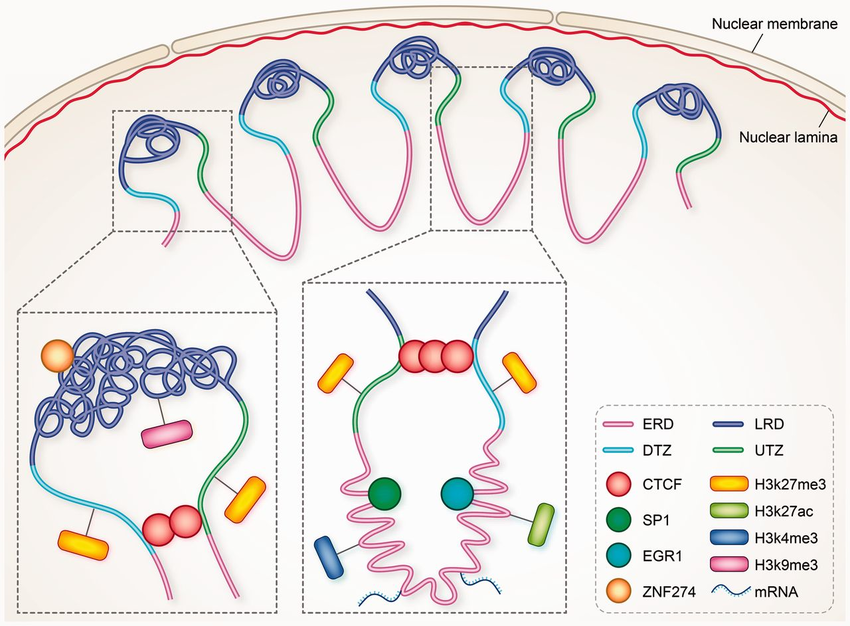
\includegraphics[width=\textwidth]{Chapters/1_introduction/figures/repdomains}
    \caption{Model of replication domains and its chromatin organization \citep{liu2016novo}.}
    \label{fig:introrepdomains}
    \end{center}
    \end{figure}

Replication is driven by replication fork which is formed when a predefined replication origin fires \citep{langston2009whither}. Replication fork usually proceeds bidirectionally, with the coordinated work of polymerases \gls{epsilon} and \gls{delta}. During the movement of the fork, polymerase \gls{epsilon} continuously synthesizes the leading strand, whereas polymerase \gls{delta} discontinuously synthesizes the lagging strand. Moreover, bidirectionality creates an asymmetric progress, so that two polymerases work on opposite strands towards different directions. In other words, in the left replicating fork, polymerase \gls{epsilon} proceeds on the plus strand, while in the right replicating fork, it progresses on the minus strand. Studies suggest that this asymmetric progress of polymerases around the associated replication origins are reflected to the mutation profiles, where lagging strands reported to harbor more mutations than leading strands \citep{haradhvala2016mutational,lujan2012mismatch,reijns2015lagging,shinbrot2014exonuclease}. Observed asymmetry on mutation profiles is explained by the error-prone bypass mechanism on the lagging strands that makes it vulnerable to mutations \citep{seplyarskiy2019error}. Other studies argued that the attachment of helicase to leading strands increases the damage response, thus leading to effective repair of the strand \citep{hedglin2017eukaryotic,yeeles2013rescuing}. Furthermore, many mutational signatures are reported to have a significant replication strand asymmetry \citep{tomkova2018mutational}.

\begin{figure}[H]
    \begin{center}
    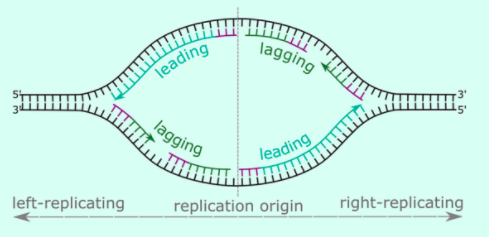
\includegraphics[width=\textwidth]{Chapters/1_introduction/figures/repfork}
    \caption{A demonstration of asymmetric synthesis of strands around replication origins \citep{tomkova2018mutational}.}
    \label{fig:introrepfork}
    \end{center}
    \end{figure}

\section{Mapping damage formation and nucleotide excision repair Events using damage sequencing (Damage-seq) and excision repair sequencing (XR-seq) methods, respectively}

Mapping of \gls{uv}-induced damages and their repair is essential to understand the role of nucleotide excision repair on mutagenesis. Since the birth of the field of \gls{dna} repair, which began with the discovery of photolyase in 1958 \citep{rupert1958photoreactivation,sancar2016mechanisms}, many methods were introduced to map \gls{dna} damage and repair \citep{li2020methodologies}. However, not until the emergence of next-generation sequencing techniques, genome-wide mapping of \gls{dna} damage and repair at single-nucleotide resolution could be performed. Today, there are several methods that can perform this task. Among these methods, Damage sequencing (\gls{dsseq}) and eXcision Repair sequencing (\gls{xrseq}) can map \gls{uv}-induced \gls{dna} damages and repair of these damages by nucleotide excision repair, respectively, which will be explained in the subsections below.

\subsection{Damage sequencing (Damage-seq)}

\gls{dsseq} mechanism can sensitively detect a variety of \gls{dna} lesions such as \gls{CPD}s, \gls{64}s, and cisplatin-DNA adducts, mainly using the \gls{rpol2} stalling to its advantage \citep{hu2016cisplatin}. In fact, the method can be adapted to any \gls{dna} damage that stalls \gls{rpol2}, where the damage-specific antibody is present \citep{sancar2016mechanisms}. After the induction of the damage, the genomic \gls{dna} is sonicated, ligated to first primers, and denaturated. Then, damage sites are immunoprecipitated by damage-specific antibodies and enriched. Following the enrichment, a biotinylated primer is annealed and extended by a polymerase called Q5 \gls{dna} polymerase, which extends the primer until it reachs the damage without synthesizing the site of the damage. Next, a second adopter is ligated to the extended primer for amplification by \gls{pcr}. Lastly, the amplified oligomers can be sequenced and analyzed (Figure \ref{fig:dsxrseq}a).      

\begin{figure}[H]
    \begin{center}
    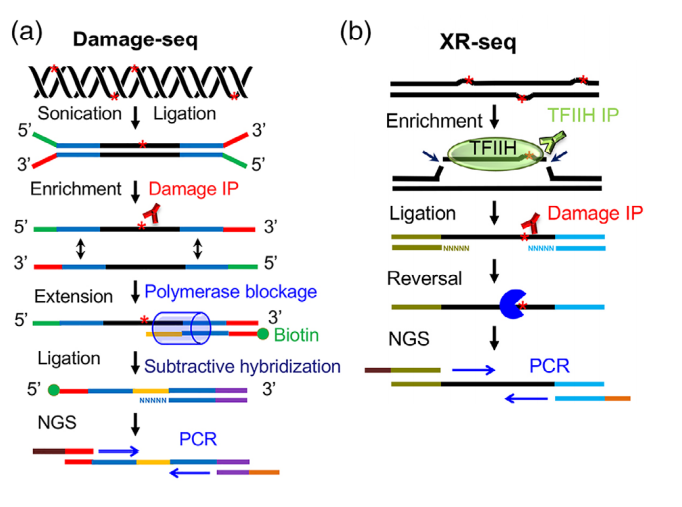
\includegraphics[width=\textwidth]{Chapters/1_introduction/figures/dsxrseq}
    \caption{Schematic representation of (a) \gls{dsseq} and (b) \gls{xrseq} \citep{li2020methodologies}.}
    \label{fig:dsxrseq}
    \end{center}
    \end{figure}

\subsection{Excision repair sequencing (XR-seq)}

\gls{xrseq} method can measure the repair of \gls{dna} damages that is coordinated by nucleotide excision repair, using the 22-30 nucleotides long exiced oligomers that are produced after the dual incision of lesion site \citep{hu2019genome,hu2016cisplatin}. Excised oligomers are immunoprecipitated by \gls{tf2h} and ligated by adaptors from both sides. Next, the oligomers are filtered according to the damage of interest by immunoprecipitating with damage-specific antibodies. Then, using photolyases, lesions of the left oligomers are reversed for a proper \gls{pcr} amplification process and the oligomers are sequenced (Figure \ref{fig:dsxrseq}b).
